\FloatBarrier
\section{Branch Behaviour of Compare-Exchange Variants} \FloatBarrier
\label{sec:CEBranchExperiment}


In Section~\ref{sec:CompareExchangeImpl} we describe different ways implementing the \texttt{Compare-Exchange} operation in such that it is possible to both eliminate the need for branches and pipeline dependencies on conditional moves.

Measuring the effect of pipeline halts from conditional moves is difficult, and their impact is heavily dependent on the underlying architecture. As such, they are to be avoided, but we will unfortunately not be able to base this on much more than good faith.

Branch mispredictions on the other hand are easily measurable and fitting for experimentation.
We measure the branch misprediction rate by running the algorithms using both the branching variant and the \texttt{xor} variant of the \texttt{Compare-Exchange} operation, subtracting the number of branch mispredictions from the \texttt{xor} variant, and divide by the number of comparisons. The reasoning for this way of obtaining branch misprediction rate being that using \texttt{xor}, we obtain the number of branch mispredictions from the overhead instructions of the algorithms, and any mispredictions that exceed this number should be caused only by comparisons.

We note that there might be some collisions in predictions between overhead and comparisons, but on a modern processor, this should be minor, especially due to the low number of branch mispredictions normally incurred by the overhead of the algorithms, as observed in Figure~\ref{fig:Performance:branchmisses} and~\ref{fig:Shellsorts:branchmisses}. 

We observe that algorithms behave differently in terms of branch misprediction rates of comparison. Note that an optimal sorting algorithm for unknown random inputs should mispredict about $50\%$ of all comparisons.

The tests are performed in the same way as those of Section~\ref{sec:Performance}, but compares two executables, one using the \texttt{xor}-based \texttt{Compare-Exchange}, and the other using the branching variant based on \texttt{std::swap}.

\subsection{Results}

\begin{figure}
\center
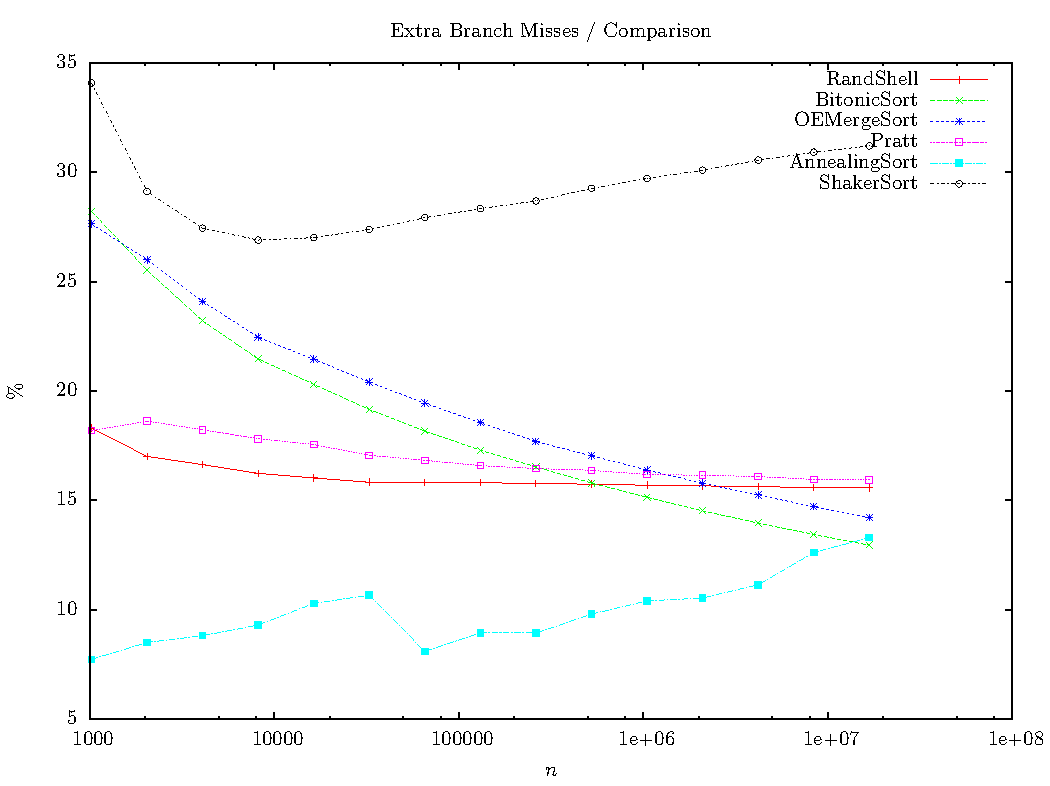
\includegraphics[width=\textwidth]{graphs/CompareExchange/branchdiff.pdf}
\caption{Branch Mispredictions of the different algorithms}
\label{fig:CompareExchange:branchdiff}
\end{figure}

Figure~\ref{fig:CompareExchange:branchdiff} shows how many of the additional branches imposed by having a data-dependent \texttt{Compare-Exchange} actually result in a branch-misprediction.

Randomized Shellsort shows a constant, but low amount of branch mispredictions. This is likely due to the fact that it makes a large random amount of comparisons, while being asymptotically optimal.

Annealing Sort also shows a low number of branch mispredictions, most likely due to performing a large amount of comparisons. As $n$ grows, we see the misprediction rate grow slightly, which might be caused by the algorithm moving slightly closer to the minimum amount of comparisons.

Bitonic Sort and Odd-Even Mergesort start off with a high number of branch mispredictions, but this number decreases as $n$ grows. This drop in misprediction is most likely caused by the additional $\Theta(\log n)$ factor of comparisons performed. When considering Bitonic Sort, the merging step will be especially graceful in branch mispredictions, as we should see them only when the two halves of the bitonic sequences cross.

Pratt's Shellsort is somewhat strange. It performs a non-optimal amount of comparisons, yet shows little improvement as $n$ increases, though it also starts low. What causes this is hard to predict, but it might be due to the way Shellsort variants often compare far-apart elements, as opposed to the somewhat local merges of Bitonic Sort and Odd-Even Mergesort

Finally, we have Shaker Sort. Shaker Sort seems to express a high and slightly growing amount of branch mispredictions. A plausible explanation for this is the close-to-optimal amount of comparisons made by Shaker Sort, and as $n$ grows, the impact of the final 1-shakes somewhat gets dampened by the growing amount of offsets in the jump sequence. Should $n$ grow fairly large, we would most likely see Shaker Sort converge towards some constant somewhere between $35$ and $50$ percent. 

\subsection{Experiment Results}

The experiment showed that one must indeed take care when implementing a \texttt{Compare-Exchange} operation on the CPU, as it will induce a large amount of branch mispredictions if it is not data-oblivious. With the big pipelines present in modern CPU architectures, this might become important.

Also, we see that the different algorithms perform a highly variable, and not always predictable, amount of branch mispredictions, as input sizes grow.